\section{Распознавание ключевых точек}
\label{sec:Chapter2} \index{Chapter2}

С развитием технологий человечество начало ставить все более разнообразные задачи, для решения которых применялись сверточные нейронные сети (convolutional neural network, CNN). Одной из таких задач оказалось распознавание ключевых точек (Keypoint Detection). При этом распознавание ключевых точек на теле человека выделилось в отдельный раздел, известный как оценка позы (Pose Estimation). Далее рассмотрим формулировку этих задач( , а также проведем обзор различных методов, которые на сегодняшний день применяются для их решения).

\subsection{Ключевые точки}

Задача распознавания ключевых точек заключается в том, чтобы обнаружить и точно локализовать определенные точки или места внутри изображения или кадра видео. Эти точки, называемые ключевыми, могут быть определены для различных объектов, таких как лица, тела человека или других структур. Например, в случае распознавания лица ключевые точки могут включать углы глаз, кончик носа, уголки рта и другие характерные особенности лица. В контексте человеческого тела ключевыми точками могут быть суставы, такие как локти, колени, плечи и так далее. Для других структур это могут быть уникальные элементы, которые помогают идентифицировать или анализировать объект.

Другими словами, ключевые точки являются опорными объектами, которые используются для определения положения и/или местонахождения объекта в пространстве. Они играют важную роль в задачах компьютерного зрения, таких как отслеживание движений, 3D-моделирование, анимация, медицинская визуализация и другие. Они могут использоваться для создания каркасов объектов, анализа их формы, измерения расстояний между различными частями и выполнения других аналитических задач.

Более точно эти объекты можно определить следующим образом: \textit{ключевые точки (КТ)} - это специфические, заранее определенные части объекта, которые имеют особое значение для дальнейшего анализа местоположения объекта на изображении. Каждая ключевая точка обычно соответствует определенной анатомической или структурной особенности, которая легко распознается и может служить ориентиром для алгоритмов обработки изображений. Иными словами, КТ необходимо обладать следующими характеристиками, чтобы можно было использовать их в качестве референсных для заданного объекта:
\begin{enumerate}
\item \textit{Уникальность}\\
Точки должны быть уникальными и отличаться от других точек на изображении
\item \textit{Инвариантность} \\
Точки должны сохранять свою идентичность при общих преобразованиях изображения, таких как вращение, масштабирование и изменения условий освещения 
\item \textit{Повторяемость} \\
Точки должны быть обнаруживаемы в разных экземплярах одного и того же объекта или сцены
\end{enumerate}

Для анализа структуры объекта и взаимосвязи между его различными КТ часто применяется схематичное описание, которое обеспечивает более наглядное визуальное представление. Этот метод помогает лучше понять анатомическую и функциональную структуру распознаваемого предмета. При этом саму схему, представляющую собой своего рода <<скелет>>, принято называть \textit{топологией}. Примеры различных топологий представлены на \autoref{fig:topology_exaples}.

\begin{figure}[h]
\begin{subfigure}[b]{0.48\textwidth}
	\centering
	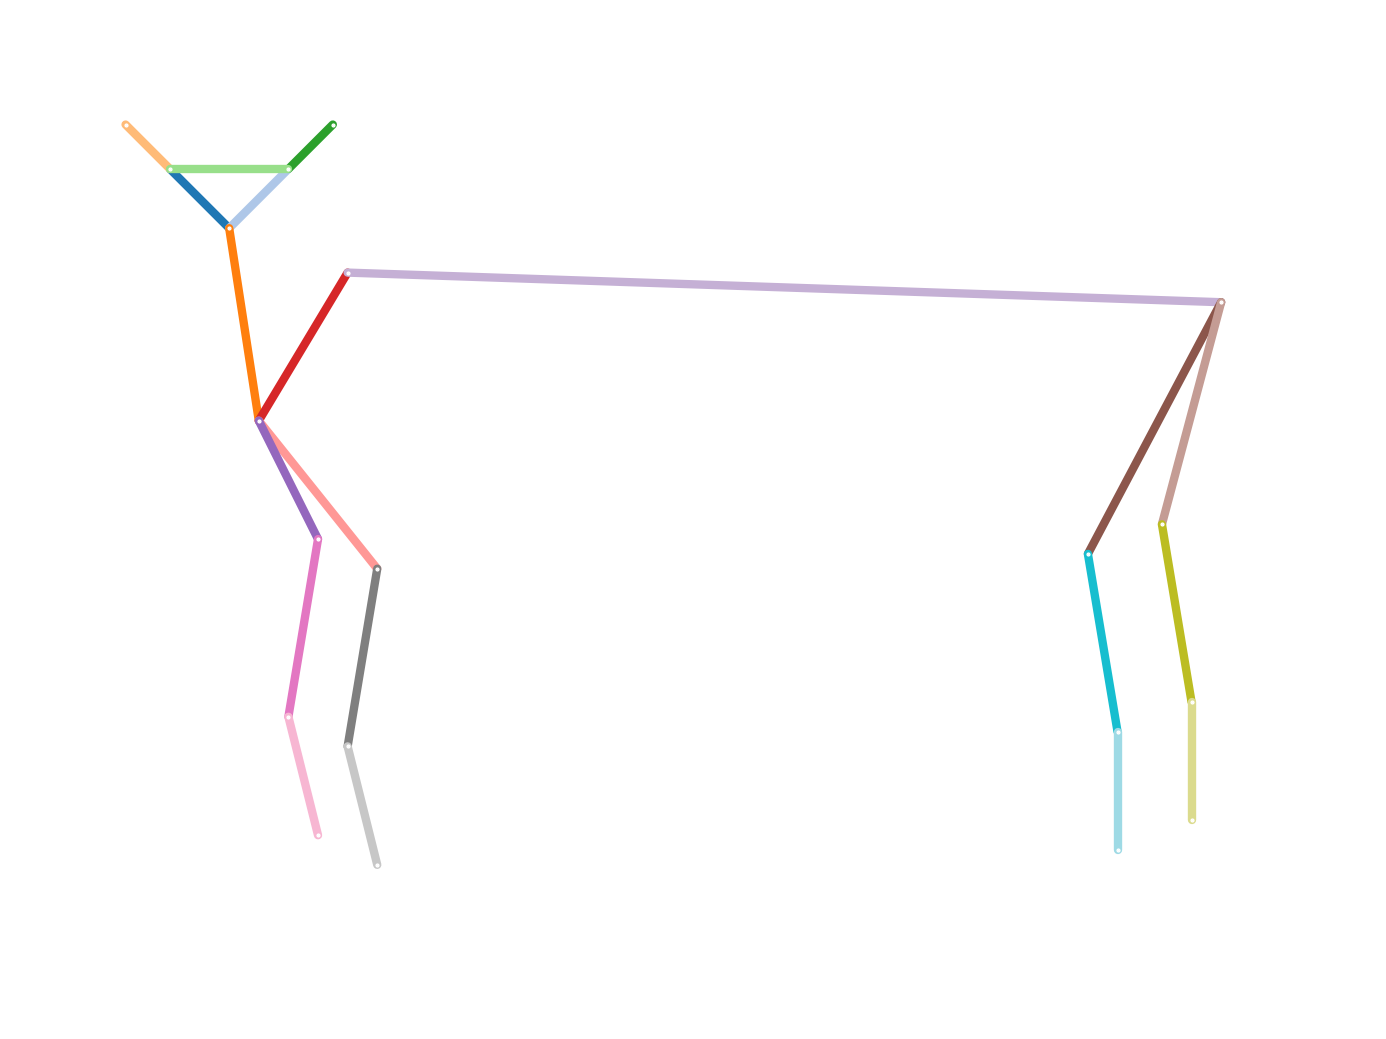
\includegraphics[width=\textwidth]{./images/plugins_animalpose.png}
	\caption{Animal Keypoints}
\end{subfigure}
\begin{subfigure}[b]{0.48\textwidth}
	\centering
	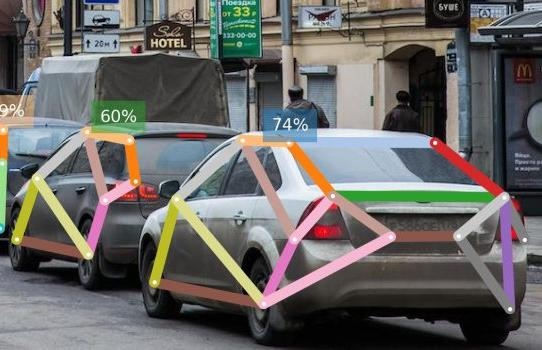
\includegraphics[width=\textwidth]{./images/car_topology.jpg}
	\caption{Car keypoints}
\end{subfigure}
	\caption{Примеры топологий объектов от OpenPifPaf \cite{OpenPifPaf2021}}
	\label{fig:topology_exaples}
\end{figure}


ВОЗМОЖНО ТУТ СТОИТ СФОРМУЛИРОВАТЬ ЗАДАЧУ РАСПОЗНАВАНИЯ КЛЮЧЕВЫХ ТОЧЕК. ОНА СФОРМУЛИРОВАНА, НО МОЖЕТ СМОГУ ДОБАВИТЬ МАТЕМАТИКИ.

\subsection{Распознавание ключевых точек на теле человека. Скелет человека}

На теле человека тоже можно выделить несколько ключевых точек, информация о которых дает возможность цифровизовать позу человека и использовать ее для аналитики с помощью методов машинного обучения. Именно для этого и была разработана задача распознавания ключевых точек на теле человека  или, как ее часто называют в англоязычной литературе, задача оценки позы человека (Human Pose Estimation).

Основной вопросом для HPE стал выбор набора ключевых точек и топологии, по которой они будут соединяться. В первых работах были представлены различные примеры топологий, некоторые примеры представлены на \autoref{fig:topology_examples}. Если точки туловища имеют большое количество пересечений, то точки головы сильно отличались: где-то учитывалось только положение головы (то есть добавлена верхняя точка головы), где-то рассматривались некоторые точки на лице, где-то голова вообще не учитывалась. Все зависело от задачи и возможностей исследователей. Позде в 2015 году Microsoft выпустило набор данных с детальным описанием 17 точек на теле человека и запустила соревнование по распознаванию этих точек \cite{COCO_dataset, COCO_topology}. Исследователей это заинтересовало и они начали адаптировать свои модели под топологию, описанную в датасете COCO \cite{COCO_dataset}. Хотя данные в наборах перестали обновлять после 2017 года, многие новые можели до сих пор оценивают свои можелли по набору данных COCO. Отсюда и получилось, что данная топология стала основной для задачи оценки позы.

\begin{figure}[t]
\centering
\begin{subfigure}[b]{.16\textwidth}
	\centering
	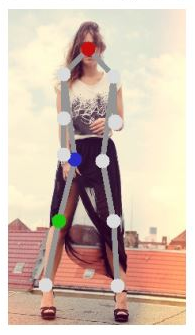
\includegraphics[width=\textwidth]{./images/regpose_topology.png}
	\caption{PDJR \cite{PDJR}}
\end{subfigure}
\begin{subfigure}[b]{.3\textwidth}
	\centering
	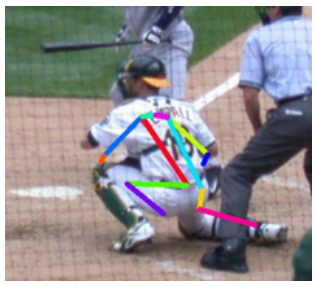
\includegraphics[width=\textwidth]{./images/deeppose_topology.png}
	\caption{DeepPose \cite{DeepPose}}
\end{subfigure}
\begin{subfigure}[b]{.455\textwidth}
	\centering
	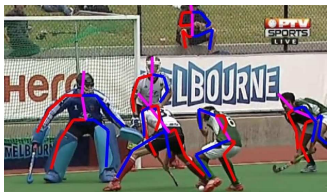
\includegraphics[width=\textwidth]{./images/alphapose_topology.png}
	\caption{AlphaPose \cite{AlphaPose}}
\end{subfigure}
\caption{Примеры различных топологий у первых решений задачи распознавания ключевых точек на теле человека}
\label{fig:topology_examples}
\end{figure}

\begin{figure}[h]
	\centering
	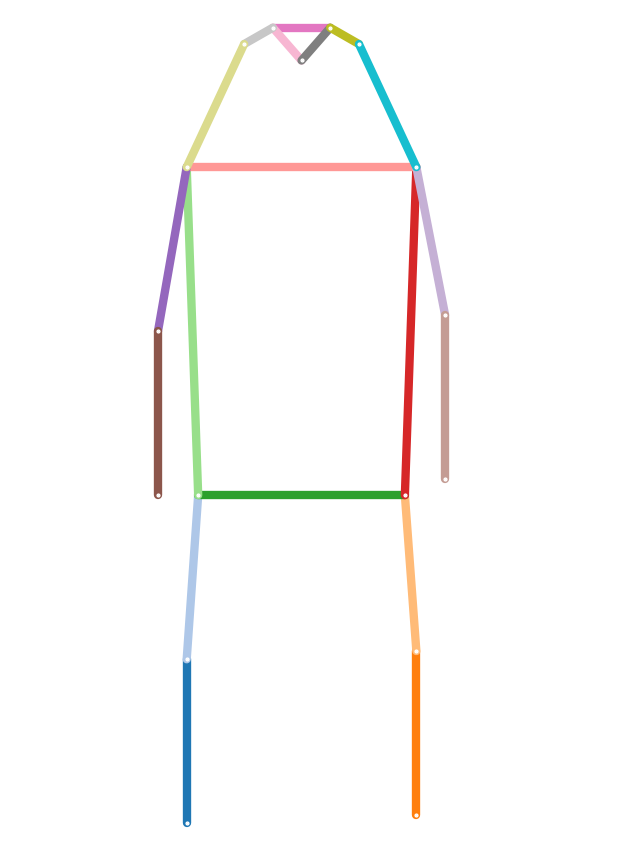
\includegraphics[width=.3\textwidth]{./images/coco_topology.png}
	\caption{Топология COCO}
	\label{fig:coco_topology}
\end{figure}

\hfill \break

Другим вопросом для описываемой задачи стал подход к распознаванию. Делать детекцию человека и уже на кропнутом изображении производить поиск или искать все возможные точки, а потом собирать их в скелет. Эти две идеи и сформировали два направления развития методов HPE. Немного о них:
\begin{enumerate}
	\item \textit{Подход сверху-вниз (англ, top-down)}\\
	Для данного этапа вам понадобится дополнительная модель детекции, которая локализует человека на изображении, выделяя его в прямоугольную область. Затем этот прямоугольник передается в модель распознавания ключевых точек. Этот подход обеспечивает высокую точность предсказания КТ, но может быть чувствителен к ошибкам на этапе обнаружения и ориентации человека в кадре, что требует дополнительной предобработки изображений.
	\item \textit{Подход внизу-вверх (англ, bottom-up)}\\
	Для данного подхода вам не нужны помощники в виде детектора, но все равно имеет два этапа в своей работе. Первоначально модель распознает все ключевые точки на полученном на вход изображении, получая таким образом карту распределения КТ по фото. А вторым шагом модель собирает все полученные точки единый скелет. При детекции нескольких людей необходимо верно сопоставить их части тела. Для этого есть несколько способом, один из которых является построение полей сходства частей тела (part affinity fields), используемый в проекте OpenPose \cite{OpenPose}.
\end{enumerate}

Но в результате обоих подходов к решению задачи на выход модели получаем массив данных [N x K x 3] в двумерном пространстве, где третьей размерностью идет предсказание видимости точки на изображении.

СТОИТ ДОБАВИТЬ ФОРМУЛ И МАТЕМАТИЧЕСКИЙ ЗАДАЧ. ПЕРЕДЕЛАТЬ ПОСЛЕДНИЙ АБЗАЦ


\newpage